\documentclass[svgnames]{article}   	% use "amsart" instead of "article" for AMSLaTeX format
%\geometry{landscape}                	% Activate for rotated page geometry

%\usepackage[parfill]{parskip}    		% Activate to begin paragraphs with an empty line rather than an indent

\usepackage{graphicx}				          % Use pdf, png, jpg, or eps§ with pdflatex; use eps in DVI mode
\setcounter{secnumdepth}{4}
\setcounter{tocdepth}{4}

%maths							                  % TeX will automatically convert eps --> pdf in pdflatex		
\usepackage{amssymb}
\usepackage{amsmath}
\usepackage{esint}
\usepackage{geometry}

%pgfplots
\usepackage{pgfplots}

%images
\graphicspath{{/Users/devaldeliwala}}					          % Activate to set a image directory 

%tikz
\usepackage{pgfplots}
\pgfplotsset{compat=1.15}
\usepackage{comment}
\usetikzlibrary{arrows}
\usepackage[most]{tcolorbox}

%Figures
\usepackage{float}
\usepackage{caption}
\usepackage{lipsum}
\newtheorem{theorem}{Theorem}

\title{Physics 89 - Introduction to Mathematical Physics}
\author{deval deliwala}
%\date{}							                % Activate to display a given date or no date

\begin{document}
\maketitle
%\section{}
%\subsection{}
\tableofcontents 					           % Activate to display a table of contents
\newpage

\noindent \textbf{Jan 17} \hrule


\section{Difference between Mathematics and Physics}
\vspace{5px}

\begin{tcolorbox}[title = Example 1 - Electrostatics]

\textbf{Math Question}
\[
  x + \frac{x^2}{2} + \frac{x^3}{3} + \frac{x^4}{4} + \dots = ? 
\]

\noindent \textbf{Math Solution}
\[
x + \frac{x^2}{2} + \frac{x^3}{3} + \dots = -\log(1-x), \hspace{10px} for -1
\leq x \leq 1
\]

So, 
\[
-1 + \frac{1}{2} - \frac{1}{3} + \frac{1}{4} - \frac{1}{5} + \dots = -\log(2)
\]

\end{tcolorbox}
\vspace{5px}
\begin{tcolorbox}[title = Example 2 - Diffusion] 
  
 \[
   f(x,y,z,t) = \text{density of diffusing material at time $t$}
 \]
 Let there exist a cube containing moles 

 \[
 \frac{\partial f}{\partial t} = D\left( \frac{\partial^2 f}{\partial x^2}
 + \frac{\partial^2 f}{\partial y^2} + \frac{\partial^2 f}{\partial z^2}\right)
 \]
 where $D$ is the \textit{diffusion coefficient}, and the diffusion equation
 describes how $f$ evolves with time \\

 \textbf{Math Question} \\

 Solve 

 \[
 \frac{\partial f}{\partial t} = D \left( \frac{\partial^2 f}{\partial x^2}
   + \frac{\partial^2 f}{\partial y^2} + \frac{\partial^2 f}{\partial
   z^2}\right)
 \]
 given initial condition 

  \[
    f(x,y,z,0) = \text{concentrated lump at the origin} 
 \]
 
 \textbf{Math Solution}
 
\[
  f(x,y,z,t) = \frac{N}{(4\pi D t)^(3/2)}e^{-\frac{x^2 + y^2 + z^2}{4Dt}}
\] \vspace{5px}

where $N$ is the number of moles released
  

\end{tcolorbox}	

\newpage
\noindent \textbf{Jan 19} \hrule
\section{Taylor Series} 

\begin{itemize}
  \item Techniques for obtaining series
  \item Estimate error, converge?     
\end{itemize}
%1

\begin{figure}[htb!]
  \centering
    \includegraphics[width = 7cm]{screenshot 35.png}
    \caption{Taylor Series Visualization}
\end{figure}


\vspace{5px} \[
  f(x) \approx f(0) + f'(0)x + \dots + \frac{1}{n!}f^{n}(0)x^n
\] \vspace{5px} 
\[
  f(x) \approx f(a) + f'(a)(x-a) + \frac{1}{2}f''(a)(x-a)^2 + ... = \sum_{k=0}^{\infty} \frac{1}{k!}f^{k} (a)
  (x-a)^k
\]

\begin{tcolorbox}[colback = red!5!white, colframe = red!50!black, title
  = Question]
  
  How good is this approximation? 

\end{tcolorbox}

\textit{ Big $O$ notation}
\vspace{5px} \[
\sum_{k=9}^{n} \frac{1}{k!}f^k(0) x^k + O(x^{n+1})
\] \vspace{5px}

\textit{ \textbf{Formally,}}

\vspace{5px} \[
  F(x) = o(x^{n+1}) \hspace{10px} \text{as } x \rightarrow 0
\] \vspace{5px}
\[
  |F| \leq C|x|^{n+1} \hspace{10px} \text{for some unexpected constant c}
\] \vspace{5px}
\[
  \lim_{x\to 0} \frac{F}{|x|^{n+1}} = 0
\] \vspace{5px}
\begin{tcolorbox}[colback = blue!5!white, colframe = blue!50!black, title
  = Example]
  \begin{gather*}
  e \approx 1.9 GeV \approx 3700 mc^2 \\\\
  \text{Special Relativity} \\
  E_k = m_0 c^2 - mc^2 = \frac{mc^2}{ \sqrt{ 1 - \frac{v^2}{c^2}}} - mc^2 \\
  \approx 0 + \frac{1}{2}mv^2 + \frac{3}{8}m\frac{v^4}{c^2} + \frac{5}{16}m
  \frac{v^8}{c^4} \\
  f(v) = \frac{1}{2}mv^2  + \frac{3}{8}m\frac{v^4}{c^2} + \dots 
  \end{gather*}
\end{tcolorbox}

\vspace{5px} \[
\frac{1}{ \sqrt{1-x}} \rightarrow \frac{mc^2}{ \sqrt{1 - \frac{v^2}{c^2}}}
\] \vspace{5px}
\[
  (1+x)^P, \hspace{10px} \text{then set $p = \frac{1}{2}$}
\]

\begin{align*}
  f(x) &= (1+x)^n  \\ f'(x) &= p(1+x)^{p-1}  \\ f^k (x)  &= p(p-1) \dots
  (p-k+1)(1+x)^{p-k} \rightarrow f^k (0) \\ &= p \dots (p-k+1) 
\end{align*}

\begin{align*}
  (1+x)^n \approx 1 + px + \frac{p(p-1)}{2!}x^2 + ... + \frac{p!}{k!(p-k)!}x^k
  = \begin{pmatrix} p \\ k \end{pmatrix}x^k
\end{align*}

\vspace{5px} \[
  \sum_{k=0}^{n} \begin{pmatrix} p \\ k \end{pmatrix} x^k \hspace{10px}
  \text{generalized binomial coefficient} 
\] \vspace{5px}
\vspace{5px} \[
  (1+x)^P = \sum_{k=0}^{n} \begin{pmatrix} p \\ k \end{pmatrix} x^k + O(x^{n+1}
\] \vspace{5px}

\begin{tcolorbox}[colback = red!5!white, colframe = red!50!black, title
  = Question]
  
  Given $\frac{1}{ \sqrt{1+x}}$ taylor series, how good is this approximation
  if $x=0.1$? 

\end{tcolorbox}
\begin{tcolorbox}[colback = blue!5!white, colframe = blue!50!black, title
  = Solution]
\vspace{5px} \[
  \text{Actual Answer} \rightarrow  \frac{1}{\sqrt{1.1}} = 0.9534626
\] \vspace{5px}
\[
  \text{Taylor Polynomials $x, x^2$} \rightarrow 1 - \frac{0.1}{2} = 0.95
  \hspace{10px} / \hspace{10px} 1 - \frac{0.5}{2} + \frac{3(0.5)^2}{8}
  = 0.95375 \hspace{10px} \text{good approx}
\] \end{tcolorbox}
\textit{ \textbf{More Taylor Series}}

\begin{align*}
  &\sin x = x - \frac{x^3}{3!} + \frac{x^5}{5!} - \frac{x^7}{7!} + \dots \\ 
  &\cos x = 1 - \frac{x^2}{2!} + \frac{x^4}{4!} - \frac{x^6}{6!} + \dots \\ 
  &e^x = 1 + x + \frac{x^2}{2!} + \frac{x^3}{3!} + \frac{x^4}{4!} + \dots \\\\
  &\cosh x = \frac{e^x + e^{-x}}{2} = 1 + \frac{x^2}{2!} + \frac{x^4}{4!}
  + \frac{x^6}{6!} + \dots \\
  &\sinh x = \frac{e^x - e^x}{2} = x - \frac{x^3}{3!} + \frac{x^5}{5!} + \dots \\ 
  %&J_o (2x) = \sum_{k=0}^{\infty} \frac{x^{2k}}{(k!)^2}(-1)^k
  %= 1 - \frac{x^2}{1!^2 + \frac{x^4}{2!^2} - \frac{x^6}{3!^2} + \dots = \text{ Bessel Function}
 \end{align*}


\subsection{Testing for Convergence}

If $ \sum_{0}^{\infty} a_n x^n \leq \infty $ converges, 

\vspace{5px} \[
\sum_{0}^{\infty} a_n (\lambda X)^n \leq \infty \hspace{10px}  \hspace{10px}
|\lambda| \leq 1
\] \vspace{5px}

Taylor Series have interval of convergence of the form 

\vspace{5px} \[
  [-L, L] \hspace{10px} (-L, L) \hspace{10px} [-L, L) \hspace{10px} (-L, L]
\] \vspace{5px}

\begin{tcolorbox}[colback = red!5!white, colframe = red!50!black, title
  = Truncated Taylor Series Approximation]
  
 \vspace{5px} \[
 R_0(x) = f(x) - f(0) = f'(c)x
 \] \vspace{5px} 

\end{tcolorbox}

%4
%remainder visualized

\begin{figure}[htb!]
  \centering
    \includegraphics[width = 10cm]{screenshot 38.png}
    \caption{Remainder Visualized}
\end{figure}



\begin{tcolorbox}[colback = blue!5!white, colframe = blue!50!black, title
  = Remainder Theorem]
 \[ 
  R_n(x) = f^{n+1} (c) \frac{x^{n+1}}{(n+1)!} \hspace{10px} \text{for some $0
  \leq c \leq x$}
\]
\end{tcolorbox}

\begin{tcolorbox}	
  
  \begin{align*}
    x &= \frac{\pi}{2} \\ 
    R &= \sin \frac{\pi}{2} - (x - \frac{x^3}{6} + \frac{x^5}{120}
    - \frac{x^7}{5040} + \frac{x^9}{362880..} + 0 ) \\
      &= f^{10}(c)\frac{x^10}{10!} \hspace{10px} 0 \leq c \leq \frac{\pi}{2}
      \\\\
    |f^{11} (c) | &= | -\cos c| < 1 \\
    |R_{10}| &\leq \frac{1}{11!} \left(\frac{\pi}{2}\right)^{11} \approx 3.6
    \times 10^{-6}
  \end{align*}

\end{tcolorbox}	
\newpage
\textbf{ \textit{Technique for Solving Taylor Series by dividing two
polynomials}}
\begin{align*}
f(x) &= a_0 + a_1x + \dots  \\
g(x) &= b_0 + b_1x + \dots \\
\frac{f(x)}{g(x)} &= (c_0 + c_1x +c_2x^2 + \dots) \\
a_0 + a_1x + \dots &= (b_0 + b_1x + \dots)(c_0 + c_1x + \dots)  \\\\
a_0 &= b_0c_0
\end{align*}

\newpage
\noindent \textbf{Jan 24} \hrule
\vspace{10px} 
\section{Complex Numbers}

\begin{itemize}
  \item Definition
  \item Functions: $\log z, \sqrt{z}, \sin z,$, etc.
  \item Applications: AC Circuits, Hydrodynamics
  \item Math Applications: $\int_{\infty}^{\infty}$
\end{itemize}

\subsection{Taylor Series}

\[
f(x) = \frac{1}{1+x^2} = \frac{1}{1-(-x^2)} = 1 - x^2 + x^4 - x^6 + - \dots
= \sum_{n=0}^{\infty} (-1)^n x^{2n}
\]

The interval of convergence for the taylor series of $\frac{1}{1+x^2}$ is from
$(-1,1)$, which is not readily apparent since 

 \[
@x \pm 1, f(x) = \frac{1}{2}
\]

%1
%taylor series of $e^{1/x^2}$

\begin{figure}[H]
  \centering
    \includegraphics[width = 7cm]{screenshot 53.png}
    \caption{taylor series of $e^{1/x^2}$}
\end{figure}



\subsection{Complex Numbers}

Introduced by \textit{Cardano} in the 1500s with the intent of solving cubic
equations.

\begin{tcolorbox}[colback = red!5!white, colframe = red!50!black, title
  = Quadratic Equations]
  
  \[
  0 = x^2 + bx + c \hspace{10px} x = -b \pm \frac{ \sqrt{b^2 - 4ac}}{2a}
  \]
\end{tcolorbox}

\begin{tcolorbox}[colback = blue!5!white, colframe = blue!50!black, title
  = Cubic Equations]
  \[
  0 = x^3 + ax + b \hspace{10px} \left(\frac{-b}{2} + \sqrt{\frac{b^2}{4}
  - \frac{a^3}{27}}\right)^{\frac{1}{3}}
  \]

  \[
    x^3 - x = 0 \rightarrow x = \frac{1}{ \sqrt{3}}\left[\sqrt{-1}^{1/3}
    + (-\sqrt{-1})^{1/3} \right]
  \]
  \begin{itemize}
    \item consistency
    \item final answer is \textbf{real}
    \item simplifies computations
  \end{itemize}  
  
\end{tcolorbox}

\paragraph{Rules of Complex Numbers}

\[
z = a + bi
\]

\[
 i^2 = -1
\]

\[
  (a + bi)(c + di) = (ac - bd) + (ad + bc)i
\]
\vspace{5px}
\begin{tcolorbox}[title = Example]

  \begin{align*}
    &(1+i)^2 = 2i \\
    &i^4 = 1
  \end{align*}

\end{tcolorbox}
\vspace{5px}

\begin{align*}
  \frac{1}{a+bi} &= \frac{(a+bi)}{(a-bi)(a+bi)} = \frac{(a-bi)}{a^2 + b^2} \\
                 &= \left(\frac{a}{a^2+b^2}\right) - \left(\frac{b}{a^2 + b^3}\right)i
\end{align*}

\subsection{Applications}

\paragraph{Hydrodynamics}

%2
%2D Diagram of Sphere from above 

\begin{figure}[H]
  \centering
    \includegraphics[width = 9cm]{screenshot 54.png}
    \caption{2D diagram of Sphere from above}
\end{figure}


\[
\vec{v}(x,y) = v_x \hat{i} + v_y \hat{j}
\]

\begin{tcolorbox}[title = Problem]	
  
  \[
  V_x, V_y = ? 
  \]
  
\end{tcolorbox}	

\begin{tcolorbox}[title = Model]

  1. Incompressible
  
   \[
     (a). \hspace{10px} 0 = \nabla \cdot \vec{v} = \frac{\partial v_x}{\partial x} + \frac{\partial
    v_y}{\partial y} 
  \] 
  2. Irrotational

  \[
    (b.) \hspace{10px} 0 = (\nabla \times \vec{v})_z = \frac{\partial v_x}{\partial x}
    - \frac{\partial v_x}{\partial y} 
  \]

\end{tcolorbox}

\begin{tcolorbox}[colback = red!5!white, colframe = red!50!black, title
  = Solving (a) and (b) ]
  
  Set of \textbf{coupled} partial differential equations (PDEs) 

  \begin{itemize}
    \item What are the Boundary Conditions? 
    \begin{itemize}
      \item an additional set of equations at the edges
    \end{itemize}
  \end{itemize}

  \begin{align*}
    &(1.) \hspace{10px} r = \sqrt{x^2 + y^2} \rightarrow \infty \hspace{10px}
    \vec{v} \rightarrow v_0 \hat{i} \\
    &(2.) \hspace{10px} \vec{v} \cdot \hat{r} = 0
  \end{align*}
  
 \textbf{Fact}: Complex Numbers \\
 Define $z = x + iy$, z is \textbf{not} the third coordinate\\
 Define $U = v_x \hat{i} - iv_y$ and $U = f(z)$ $\rightarrow$ Equations (a.)
 and
 (b.) are automatically satisfied. 

\end{tcolorbox}

\begin{tcolorbox}[colback = blue!5!white, colframe = blue!50!black, title
  = Solution]
  \[
  U = v_0\left(1-\frac{R^2}{z^2}\right)
  \]

  \[
  \frac{1}{z} = \frac{1}{x+iy} = \frac{x-iy}{x^2 + y^2}
  \]
  \[
  \frac{1}{z^2} = \frac{x^2 - y^2 - 2ixy}{(x^2 + y^2)^2}
  \]
  \[
  v_x = v_0 - \frac{v_0R^2(x^2 - y^2)}{(x^2 + y^2)^2}
  \]
  
\end{tcolorbox}

\paragraph{The Complex Plane}

%3
\begin{figure}[H]
  \centering
    \includegraphics[width = 10cm]{screenshot 55.png}
    \caption{complex plane}
\end{figure}

\begin{figure}[H]
  \centering
    \includegraphics[width = 7cm]{screenshot 56.png}
    \caption{quadrant's of complex plane in polar coordinates}
\end{figure}




\paragraph{Euler's Identity}

\[
  \cos \theta + i \sin \theta = e^{i\theta}
\]
\begin{align*}
  e^{x} &= 1 + \frac{x}{1} + \frac{x^2}{2} + \frac{x^3}{3!} + ...
  \sum_{n=0}^{\infty} \frac{x^n}{n!} \\
  e^{iy} &= 1 + \frac{iy}{1} - \frac{y^2}{2!} - \frac{iy^3}{3!} + \frac{y^4}{4!}
  + \dots \\
         &= \left(1 - \frac{y^2}{2!} + \frac{y^4}{4!} + \dots \right) + \left(\frac{y}{1}
- \frac{y^3}{3!} + \dots \right)i = \cos y + i \sin y 
\end{align*}

\begin{tcolorbox}[title = Euler's Identities]
  \begin{align*}
    e^{i\pi} &= -1 \\
    1 = e^{2\pi i} &= e^{2\pi n i} \hspace{10px} n = 0, \pm 1, \pm 2, \dots
\end{align*}

\end{tcolorbox}

\[
\log z = ?
\]
\begin{align*}
  z &= re^{i\theta} \\
  \log z &= \log r + i(\theta + 2 \pi n)
\end{align*}

\[
\sqrt{z}
\]
\begin{align*}
  \sqrt{re^{iz}} &= \sqrt{r} e^{i\theta / 2} \\
                 &= \sqrt{r}e^{\frac{i(\theta + 2\pi)}{2}}\\
                 &= -\sqrt{r} e^{i\theta / 2}
\end{align*}

\paragraph{Trigonometric Functions}

\[
  \cos z = \frac{e^{iz} + e^{-iz}}{2}
\]
\[
  \sin z = \frac{e^{iz} - e^{-iz}}{2i}
\]
\[
  cos(iy) = \frac{e^{-y} + e^{y}}{2} = \cosh y
\]
\[
  sin(iy) = i\frac{e^y - e^{-y}}{2} = i\sinh y
\]

\subsection{Hyperbolic Functions}

\[
\tanh = \frac{\sinh y}{\cosh y}
\]

Everything is \textbf{Real} from now on.

\paragraph{Identities} 

\begin{align*}
  \sinh (\alpha + \beta) &= \sinh \alpha \cosh \beta + \cosh \alpha + \sinh
  \beta \\
  \cosh (\alpha + \beta) &= \cosh \alpha \cosh \beta + \sinh \alpha + \sinh
  \beta \\
  \tanh (\alpha + \beta) &= \frac{\tanh \alpha + \tanh \beta}{1 + \tanh \alpha
  \tanh \beta}
\end{align*}

\paragraph{Applications to Special Relativity}

\textbf{Relativistic Addition to Velocities}

%4 
%A train moving, with a car moving inside of it, what would an observer
%calculate for the speed of the interior car? 

\begin{figure}[H]
  \centering
    \includegraphics[width = 6cm]{screenshot 57.png}
    \caption{a train moving with a car moving inside of it, what would an
    observer calculate for the speed of the interior car?}
\end{figure}



\[i
 W = \frac{u + v}{1 + \frac{uv}{c^2}} = c \frac{\tanh \alpha - \tanh\beta}{1
 + \tanh \alpha + \tanh \beta} = c\tanh(\alpha + \beta) 
\]
%5
%Rapidity - Using hyperbolic tanget establishes the bounds of velocity as c and
%-c

\begin{figure}[H]
  \centering
    \includegraphics[width = 8cm]{screenshot 58.png}
    \caption{rapidity - using hyperbolic tangent establishes the bounds of
    velocity as $c$ and $-c$}
\end{figure}

\newpage
\noindent \textbf{Jan 26} \hrule
\vspace{10px}
Functions of Complex Variables

\begin{itemize}
  \item Cauchy - Riemann Eqns
  \item Taylor Series
  \item  $\int_{-\infty}^{\infty}$
\end{itemize}
\vspace{5px}
\begin{itemize}
  \item Singularities, Poles, Residue
\end{itemize}

The Complex Conjugate
%1

\begin{figure}[H]
  \centering
    \includegraphics[width = 5cm]{screenshot 73.png}
    \caption{graphing complex numbers}
\end{figure}


\[
\bar z = a - bi \hspace{10px} z \bar z = a^2 + b^2 = |z|^2
\]

Functions of $z = x + iy$ 

\begin{align*}
  ReZ = x \\
  ImZ = y \\
  |z| = \sqrt{x^2 + y^2} \\
  \bar = z = x - iy 
\end{align*}

\begin{tcolorbox}[title = Analytic Functions]

  \begin{align*}
    \frac{1}{z} \\
    z^2 \\
    e^z \\
    \sin z \\
    \cos z
  \end{align*}

\end{tcolorbox}

\begin{align*}
  f(z) = u + iv \\\\
  u = u(x,y) \\
  v = v(x,y) 
\end{align*}\\\\
Analytic Functions are the functions where you can write 

\vspace{5px} \[
f(z + \Delta z) - f(z) = f'(z)\Delta z + O(\Delta z^2) \hspace{10px} \Delta
z \rightarrow 0
\] \vspace{5px}
\textit{ \textbf{Note}}
\[
f(x + \Delta x, y + \Delta y) - f(x,y) = \left( \frac{\partial f}{\partial
  x}\right) \Delta x + \left( \frac{\partial f}{\partial y} \right) \Delta
  y + \dots 
\]

\textit{ \textbf{Check}}

\[
  e^{z + \Delta z} = e^ze^{\Delta z} = e^z ( 1 + \Delta z + \dots)
\]
\[
  e^{z + \Delta z} - e^z = e^z \delta z + \dots = f''(z) \delta z + \dots 
\]
\vspace{5px}
Therefore, $e^{z + \Delta z}$ is  \textit{analytic}.  However, 
\[
\bar z + \Delta \bar z - \bar z = \bar \Delta z
\]
\[
\Delta z = \Delta x \rightarrow \bar \Delta z = (1) \Delta z \hspace{10px}
\text{Horizontal}
\]
\[
\Delta z = i \Delta y \rightarrow \bar \Delta z = -i\Delta y = (-1)\Delta
z \hspace{10px} \text{Vertical}
\]
\vspace{5px}
\hrule
\begin{align*}
  &f(z) = u + iv \\\\
  &\frac{f(x + \Delta x, y) - f(x)}{\Delta x} = f'(z) \\\\
  &\frac{f(x, y + \Delta y) - f(x,y)}{i\Delta y} = f'(z) = \frac{\partial
  f}{\partial y} \frac{1}{i}
\end{align*}

\vspace{5px}
\hrule

\begin{align*}
  &\frac{\partial f}{\partial x}  = \frac{1}{i} \frac{\partial f}{\partial y} \\ 
  &\left( \frac{\partial u}{\partial x}\right) + i\left( \frac{\partial
    v}{\partial x} \right) = \frac{1}{i} \left[\left( \frac{\partial
      u}{\partial y} \right) + i \left( \frac{\partial v}{\partial y}
  \right)\right] \\ 
  &= \frac{\partial v}{\partial y}  - i \frac{\partial u}{\partial y} 
\end{align*}


\begin{tcolorbox}[colback = blue!5!white, colframe = blue!50!black, title
  = Cauchy Riemann Equations] 
  \begin{align*}
    &\frac{\partial u}{\partial x} = \frac{\partial v}{\partial y} \\
    &\frac{\partial u}{\partial y} = - \frac{\partial v}{\partial x} 
  \end{align*}

\end{tcolorbox}
\vspace{5px}
\textit{ \textbf{Example}}


\begin{align*}
  f(z) = x^2 - y^2 + 2i xy \\\\
  &u = x^2 - y^2 \\
  &v = 2xy \\\\
  &\frac{\partial u}{\partial x} = 2x = \frac{\partial v}{\partial y} \\\\
  &\frac{\partial u}{\partial y} = -2y = - \frac{\partial v}{\partial x} 
\end{align*}
%2

\begin{figure}[H]
  \centering
    \includegraphics[width = 8cm]{screenshot 74.png}
    \caption{a region in the complex plane}
\end{figure}



\paragraph{Taylor Series}

\[
  f(z) = \sum_{n=0}^{\infty} a_n z^n \hspace{50px} \text{converges if analytic}
\]

Given a constant $\lambda$
\[
0 < \lambda < 1
\]
\[
f(\lambda z) = \sum_{n=0}^{\infty} a_n (\lambda z)^n \hspace{50px}
\text{definitely converges}
\]
\[
| a_n z^n \lambda^n | = |a_n z^n | |\lambda|^n 
\]

Let $\lambda = re^{i\theta}$, $0 < r < 1$,  $|\lambda| < 1$

%3
%Taylor Series Disk of Convergence

\begin{figure}[H]
  \centering
    \includegraphics[width = 7cm]{screenshot 75.png}
    \caption{disk of convergence of power series}
\end{figure}

\begin{figure}[H]
  \centering
    \includegraphics[width = 7cm]{screenshot 76.png}
    \caption{disk of convergence is disk with maximum radius inside $R$}
\end{figure}





\mbox{} \\
\hrule
\vspace{10px} 
\textit{ \textbf{Example}}

\[
f(x) = \frac{1}{x^2 + 1}
\]
\[
f(z) = \frac{1}{z^2 + 1}
\]

%5
%Using complex instead of real to calculate interval of convergence
\begin{figure}[H]
  \centering
    \includegraphics[width = \linewidth]{screenshot 77.png}
    \caption{using complex number instead of real numbers to calculate interval
    of convergence}
\end{figure}



\textbf{ \textit{Example}}

\[i
f(z) = \log(z) 
\]
%6
\begin{figure}[H]
  \centering
    \includegraphics[width = 7cm]{screenshot 78.png}
    \caption{graph of complex log to determine convergence}
\end{figure}




\paragraph{Path Integrals}

\begin{align*}
  \int_{\infty}^{\infty} \left(\frac{\sin x}{x} \right) dx = \pi \\
  \int_{-\infty}^{\infty} \frac{dx}{x^2 + 1} = \arctan
  x \big|_{-\infty}^{\infty} = \pi
\end{align*}

%7
\begin{figure}[H]
  \centering
    \includegraphics[width = 8cm]{screenshot 79.png}
    \caption{path $P$}
\end{figure}


\textbf{Technique}

Parametrize P from $ 0 < t < \pi$ as  $z(t)$

%8
\begin{figure}[H]
  \centering
    \includegraphics[width = 6cm]{screenshot 80.png}
    \caption{example of parameterizing $z(t)$}
\end{figure}


\[
\int_P f(z)dz = \int_a^b f(z(t)) \left( \frac{d z}{d t} \right)dt 
\]
\begin{align*}
  &f(z) = z^3 \\
  &\frac{d z}{d t} = iRe^{it} \\
  &f(z(t)) = \left(Re^{it} \right)^3 = R^3e^{3it}
\end{align*}

\textbf{Collect}  
\begin{align*}
  \int_0^\pi f(z(t) \left( \frac{d z}{d t}  \right) dt &= \int_0^\pi R^3e^{3it}
  (iRe^{it})dt \\
                                                       &= i R^4 \int_0^\pi e^{4 i t} = \frac{iR^4}{4i} e^{4it} \Big|_0^\pi = 0 \\
  e^{4\pi i} &= 1
\end{align*}

\paragraph{Contour Integrals}
%9
\begin{figure}[H]
  \centering
    \includegraphics[width = 5cm]{screenshot 81.png}
    \caption{contour integral path}
\end{figure}


\vspace{5px}
Contour Integrals $ = 0$ for any analytic function that is analytic for the
entire region C

\begin{align*}
  &\oint_C f(z) dz = 0 \\
  &= \int_0^{2\pi} R^n e^{nit} \frac{dz}{dt}dt \\
  &= \int_0^{2\pi} R^n e^{nit} iRe^{it} dt  \\
  &= iR^{n+1} \int_0^{2\pi} e^{i(n+1)t} dt \\
  &= \frac{iR^{n+1}}{i(n+1)} e^{i(n+1)t} \Big|_0^{2\pi} = 0
\end{align*}

\textbf{Effect of Singularities}

Let $n = -1$
\begin{align*}
  f(z) = \frac{1}{z} \\
  \oint_C \frac{dz}{z} = iR^{n+1} \int_0^{2\pi} e^{i(n+1)t} dt \\
  = i \int_0^{2\pi} dt = 2\pi i \neq 0
\end{align*}

\begin{figure}[H]
  \centering
    \includegraphics[width = 7cm]{screenshot 82.png}
    \caption{Fundamental Theorem of Contour Integrals}
\end{figure}



\begin{tcolorbox}	
  
  \[
  \int_a^b f(z) dz = F(b) - F(a) 
  \]
  
  
\end{tcolorbox}	
\mbox{} \\
\textbf{Example}

\[
  f(z) = \frac{1}{z^2 + 1} \hspace{30px} \alpha = i
\]

\begin{align*}
  = \frac{1}{(z-i)(z+i)} = \frac{1}{z-i} \left(\frac{1}{z+i}\right)
\end{align*}

\begin{align*}
  f(z) = \frac{g(z)}{z - \alpha} \\\\
  f(z) = \frac{1}{z-\alpha} [g(\alpha) + (z-\alpha)g'(\alpha) + \dots] \\
  = \frac{g(\alpha}{z - \alpha} + g'(\alpha) + \dots  
\end{align*}

\begin{tcolorbox}	
  
  \[
  \oint_C f(z)dz = \oint_C' f(z)dz = \oint_D f(z)dz = \oint
  \frac{g(\alpha)}{z-\alpha} dz
  \]

\end{tcolorbox}	

\newpage
\noindent \textbf{Jan 31} \hrule
\vspace{10px}
Main Topic

\begin{itemize}
  \item Tensors (Vectors First)
\end{itemize}

\paragraph{Analytic Functions} 

\[
  f(z) = x + iy = \sum_{n=0}^{\infty} a_n (z-\alpha)^n
\]
Taylor series around $\alpha$ -- Disk of Convergence


\paragraph{Cauchy Riemann Equations} 

\begin{align*}
  &f(z) = u + iv \\\\
  u = Ref \\
  v = Imf
\end{align*}

\begin{tcolorbox}[colback = blue!5!white, colframe = blue!50!black, title
  = Cauchy Riemann Equations]

  \begin{align*}
    &\frac{\partial u}{\partial x}  = \frac{\partial v}{\partial y}  \\
    &\frac{\partial u}{\partial y} = -\frac{\partial v}{\partial x} 
  \end{align*}
  

\end{tcolorbox}

\paragraph{Hydrodynamics} 

%1
\begin{figure}[H]
  \centering
    \includegraphics[width = 14cm]{screenshot 91.png}
    \caption{velocity field of a fluid obeying Cauchy-Riemann Equations}
\end{figure}



If $v(z)$ is analytic 

\begin{itemize}
  \item Incompressible: $ \frac{\partial v_x}{\partial x}  + \frac{\partial
    v_y}{\partial y} = 0$ 
  \item Irrotational: $ \frac{\partial v_x}{\partial y} - \frac{\partial
    v_y}{\partial x} = 0$
\end{itemize}


\paragraph{Contour Integrals}
\mbox{}\\
%2
\begin{figure}[H]
  \centering
    \includegraphics[width = 14cm]{screenshot 92.png}
    \caption{Equation for contour integrals with a singularity: $2\pi i \sum_n
    Res_{z \to \alpha} f$}
\end{figure}



%3
\begin{figure}[H]
  \centering
    \includegraphics[width = 5cm]{screenshot 93.png}
    \caption{it's called a singularity / simple pole because the magnitude of
    the function approaches infinity at $\alpha$}
\end{figure}



%4
\begin{figure}[H]
  \centering
    \includegraphics[width = 15cm]{screenshot 94.png}
    \caption{Examples of integrals that are easier with Contour Integration}
\end{figure}


\textit{ \textbf{Theorem}} 

\[
\sum_{n=0}^{\infty} a_n (z-\alpha)^n \text{ converges with nonzero radius of
convergence for every $\alpha \in R$}
\]
\[
f(z) \text{ is a analytic function in region } R. 
\]
\paragraph{Computing Res $f$ at $\alpha$} 

 \[
f(z) = \frac{g(z)}{h(z)} \approx \frac{g(\alpha)}{(z-\alpha)h'(\alpha)}
= \frac{g(\alpha) / h'(\alpha)}{z - \alpha} = \frac{R}{z - \alpha}
\]
\section{Tensors} 

\subsection{Vectors first} 

\textbf{Goal} 

Geometric notion of a vector --- Algebraic notion of a vector

%5
\begin{figure}[H]
  \centering
    \includegraphics[width = 14cm]{screenshot 95.png}
    \caption{matrix vector visualization}
\end{figure}


\vspace{5px}
\[
\begin{pmatrix} 
\cos\theta & \sin\theta \\
-\sin\theta & \cos\theta 
\end{pmatrix}
\]
The Rotation Matrix
\vspace{10px} 
\begin{tcolorbox}	
  
  \[
    A'_j = \sum_{i=1}^{2} R_{ji} A_i
  \]
  
  

\end{tcolorbox}	

\textit{Example}

\begin{align*}
  A'_2 = \sum_{i=1}^{2} R_{2i} A_i &= R_{21} A_1 + R_{22} A_2 \\
                                   & = -\sin\theta A_1 + \cos\theta A_2
\end{align*}

\begin{figure}[H]
  \centering
    \includegraphics[width = 15cm]{screenshot 96.png}
    \caption{Changing Coordinates - Rotation Matrices}
\end{figure}




\textbf{Tensors} 
\mbox{}\\\\
Made up of components $ \frac{\partial v_i}{\partial x_j} $.
\\\\ Each derivative component of the tensor has different values from different coordinate systems. 
\mbox{}\\\\
\textbf{Simple Tensors}
\mbox{}\\

Two Vectors
\[ \vec{A}, \vec{B} \]
Then 
\[
  T_{ij} = A_i B_j 
\]

%7
\begin{figure}[H]
  \centering
    \includegraphics[width = 7cm]{screenshot 97.png}
    \caption{Prime vs. Unprimed coordinate axes}
\end{figure}



\[
  T'_{ij} = A'_i B'_j = \left(\sum_{k=1}^2 R_{jk} A_k \right)\left( \sum_{l
  = 1}^2 R_{jl} B_l \right)
\]

\[
  = \sum_{k=1}^2 \sum_{l=1}^2 R_{ik} R_{jl} A_k B_l
\]

\begin{tcolorbox}[title = Tensor Transformation Law]

\[
  T'_{ij} = \sum_{k=1}^{2} \sum_{l=1}^{2} R_{ik} R_{jl} T_{kl}
\]

\end{tcolorbox} 
\vspace{10px} 
\textit{ \textbf{Example}}: Theory of Elasticity 
\\\\


%8
\begin{figure}[H]
  \centering
    \includegraphics[width = \linewidth]{screenshot 98.png}
    \caption{Parallel forces on surfaces perpendicular to their axis}
\end{figure}



\begin{align*}
  &\vec{S_1} = \lim_{\Delta y \Delta z \to 0} \frac{\vec{F}_x}{\Delta y \Delta 
  z} \\
  &\vec{S_2} = \lim \frac{\vec{F_y}}{\Delta x \Delta z}\\
  &\vec{S_3} = \lim \frac{\vec{F_z}}{\Delta x \Delta y} \\\\
  & S_{ij} = (\vec{S_i})_j \hspace{10px} i,j = 1,2,3,\dots \hspace{10px}
  \text{Stress Tensor} 
\end{align*}

Using the stress tensor: 

%9
\begin{figure}[H]
  \centering
    \includegraphics[width = 15cm]{screenshot 99.png}
    \caption{to calculate the force on the triangle, you can sum the forces on
    the edges $a,b,c$ of the triangle}
\end{figure}



The forces $S_{11}, S_{22}, S_{33}$ are "pushing forces"  

The forces $S_{12}, S_{23}, S_{13}, \dots$ are "shear forces" 

\paragraph{Dot Product} 

%10
\[
  \vec{A} \cdot \vec{B} = |\vec{A}||\vec{B}|\cos\phi 
\]

In components, 

\vspace{5px} \[
  \vec{A} \cdot \vec{B} = \sum_{i=1}^{3} A_i B_i = \sum_{i=1}^3 \sum_{j=1}^3
  C_{ij} A_i B_j 
\] \vspace{5px}

\[
  \delta_{ij} =  C_{ij} = 1 \hspace{10px} i = j 
\]
\[
  \delta_{ij} = C_{ij} = 0 \hspace{10px} i \neq j
\]

\[
\begin{pmatrix} 
1 & 0 & 0 \\
0 & 1 & 0 \\
0 & 0 & 1 
\end{pmatrix} 
\]
Kronecker Delta Symbol Tensor 
\mbox{}\\

Checking Tensor Transformation Law: 

\[
  \delta'_{ij} = \sum_{k=1}^2\sum_{l=1}^2 R_{ik} R_{jl} \delta_{kl}
\]

is correct for any rotation in any dimension



\paragraph{Cross Product} 

\begin{align*}
  \vec{A} \times \vec{B} = \begin{vmatrix} 
    \hat{i} & \hat{j} & \hat{k} \\
  A_1 & A_2 & A_3 \\
  B_1 & B_2 & B_3 
  \end{vmatrix} \\\\
  (\vec{A} \times \vec{B})_i = \sum_{j=1}^3\sum_{k=1}^3 C_{ijk} A_j B_k \\\\
  &C_{ijk} = 1 \hspace{10px} ijk = (123), (231), (312) \\
  &C_{ijk} = -1 \hspace{10px} ijk = (132), (321), (213) \\
  &C_{ijk} = 0 \hspace{10px} i = j, i = k, j = k
\end{align*}

The Levi - Civita Tensor


\newpage
\noindent \textbf{Feb 2} \hrule
\vspace{10px}
\textit{ \textbf{HW2 Oscillations}} 
\mbox{}\\\\
Oscillations - All equations ~ $\sin (\omega t + \phi) = A \sin \omega
t + B\cos \omega t$ 

%1
\begin{figure}[H]
  \centering
    \includegraphics[width = \linewidth]{screenshot 122.png}
    \caption{HW2 Problem Set Q2 Analogy to AC circuits}
\end{figure}




\paragraph{Tensor Recap} 

Collection of components $T_{ij}$ 

%2
\begin{figure}[H]
  \centering
    \includegraphics[width = 10cm]{screenshot 123.png}
    \caption{Rotation Matrices}
\end{figure}



\begin{tcolorbox}[colback = red!5!white, colframe = red!50!black, title
  = Transformation Theory]
  
  \[
    T_{ij} = \sum_{k=1}^{2} \sum_{l=1}^{2} R_{ik}R_{jl}T_{kl}
  \]
  
  

\end{tcolorbox}


\begin{align*}
  \vec{A} \cdot \vec{B} = \sum_{k=1}^2 A_k B_k 
\end{align*}

\subsection{Einstein Convention}

\[ \vec{A} \cdot \vec{B} = A_k B_k \hspace{10px} \text{Dropping the Summation
- implied sum regardless}
\]

\paragraph{Tensor Equations}

\[
  S_{ij} = T_{ij} + \sum_{k=1}^2 W_{ik}P_{jk}
\]
\[
  S'_{ij} = T'_{ij} + W'_{ik} P'_{jk}
\]

\textbf{ \textit{Hydrodynamics}}
\mbox{}\\\\
\noindent $S_{ij} = \text{stress tensor}$
\mbox{}\\
$W_{ij} = \frac{\partial v_j}{\partial x_j} = \partial_i v_j$ 
\mbox{}\\
$S_{ij} = \alpha (\partial_i v_j + \partial_j v_i) + \beta (\partial_k
v_k)\delta_{ij}$

\[
  \sum_{k=1}^{3} \partial_k v_k = (\nabla \cdot \vec{v})
\]

\textit{ \textbf{Cross Product}}
\[
(\vec{A} \times \vec{B})_k = \sum_{l=1}^{3} \sum_{m=1}^{3}  \varepsilon_{klm}
A_l B_m
\]
\[
  (\vec{A} \times \vec{B})_3 = A_1B_2 - A_2B_1 
\]

\[
  E'_{klm} = R_{ki} R_{mn} E_{ijn} \hspace{10px} \text{Einstein notation}
\]
\[
 \sum_{i=1}^{3}  \sum_{j=1}^{3}  \sum_{n=1}^{3}   
\]

\subsection{Uses of Tensors}  

\begin{align*}
  [\vec{A} \times (\vec{B} \times \vec{C})]_k = (\vec{A} \cdot
  \vec{C})\vec{B}_k
  - (\vec{A} \cdot \vec{B})\vec{C}_k        
\end{align*}

Given 

\[
  (\vec{A} \times \vec{B})_k = \varepsilon_{klm} A_l B_n 
\]
\begin{align*}
  [\vec{A} \times (\vec{B} \times \vec{C})]_k &= \varepsilon_{klm} A_l (\vec{B}
  \times \vec{C})_m \\
                                              &= \varepsilon_{klm} A_l
                                              \varepsilon_{mij} B_iC_j \\
                                              &= (\delta_{kj} \delta_{lj}
                                              - \delta_{kj}\delta_{li})A_lB_iC_j
                                              \\
                                              &= \delta_{ki}\delta_{lj}A_l B_i
                                              C_j - \delta_{kj} \delta_{li}
                                              A_lB_iC_j \\
                                              &= A_j C_jB_k
\end{align*}

\begin{align*}
  &\sum_{m=1}^{3} \varepsilon_{klm} \varepsilon_{mij} = \delta_{ki} \delta_{lj}
  - \delta_{kj} \delta_{li} \\\\
  &\sum_{l=1}^{2} \delta_{lj}A_l = 0A_1 + 1A_2 + 0A_3 = A_j  \hspace{10px}
  \text{since $\delta_{lj} =1$ only if $l=j$} 
\end{align*}

\section{Vector Spaces}

\begin{figure}[H]
  \centering
    \includegraphics[width = 8cm]{screenshot 124.png}
    \caption{Vector space properties example}
\end{figure}


\[
  \vec{A}, \vec{B} \rightarrow \vec{A} + \vec{B} 
\]
\[
  \vec{A} \rightarrow \lambda \vec{A}
\]
\subsection{Complex Vector Spaces}

\[
  \vec{A} = \begin{pmatrix} A_1 \\ A_2 \end{pmatrix}, \vec{B} = \begin{pmatrix}
B_1 \\ B_2 \end{pmatrix} 
\]
\[
  \vec{A} + \vec{B} = \begin{pmatrix} 
  A_1 + B_1 \\
  A_2 + B_2 
  \end{pmatrix} 
\]

\paragraph{Quantum Computing} 

\begin{align*}
  0 \rightarrow \begin{pmatrix} 1 \\ 0 \end{pmatrix} \\
  1 \rightarrow \begin{pmatrix} 0 \\ 1 \end{pmatrix}
\end{align*}

%4

\begin{figure}[H]
  \centering
    \includegraphics[width = 10cm]{screenshot 125.png}
    \caption{Analogy to Lasers in Quantum Computing}
\end{figure}



\[
\begin{pmatrix}
  1 \\ i 
\end{pmatrix} = \vec{A} + i\vec{B} \hspace{10px} \text{circularly polarized}  
\]
%5
\begin{figure}[H]
  \centering
    \includegraphics[width = 6cm]{screenshot 126.png}
    \caption{Quick vectors geometric fact}
\end{figure}



Functions $f(x)$ are also vector spaces since 

\begin{align*}
  & f(x) + g(x) = h(x) \\
  & \lambda f(x) 
\end{align*}

\paragraph{Linearly Independent Vectors} 
\begin{figure}[H]
  \centering
    \includegraphics[width = 12cm]{screenshot 127.png}
    \caption{Linearly Dependent and Independent Vectors}
\end{figure}



\begin{align*}
  &\vec{A_1}, \vec{A_2}, \dots, \vec{A_n} \\ 
  &0 = \lambda_1 \vec{A_1} + \dots + \lambda_n \vec{A_n} \hspace{10px}
  \text{linear combination of $A_1 \rightarrow A_n$}
\end{align*}

\paragraph{Inner Product} 

\[
  \vec{A} \cdot \vec{B} = \sum_{k=1}^{n} A_k B_k 
\]
\[
\langle \vec{A} \big| \vec{B} \rangle = \sum_{k=1}^{n} \bar A_k B_k
\]

\[
|\vec{A}|^2 = \langle \vec{A} \big| \vec{A} \rangle = \sum_{k=1}^{3} |A_k|^2 \geq 0 
\]

\begin{align*}
  &\langle \vec{A} \big| \vec{B} + \vec{C} \rangle = \langle \vec{A} \big|
  \vec{B}\rangle + \langle \vec{A} \big| \vec{C}\rangle \\
  &\langle \vec{A} \big| \lambda \vec{B} \rangle = \lambda \langle \vec{A}
  \big| \vec{B} \rangle \\
  & \langle \vec{B} \big| \vec{A} \rangle = (\langle \vec{A} \big| \vec{B}
  \rangle )\ast
\end{align*}

\begin{align*}
  |\langle \vec{A} \big| \vec{B} \rangle |^2 \leq |\vec{A}|^2 |\vec{B}|^2 \hspace{10px}
  \text{Cauchy-Schwartz Inequality}
\end{align*}

\paragraph{Algorithm}

\[
f_1, f_2, f_3
\]

 \[
\vec{e_1} = \frac{\vec{f_1}}{|f_1|} 
\]
\[
\vec{e_2} \rightarrow \vec{u_2} = f_2 - (\vec{e_1}\vec{f_2})\vec{e_1} + \dots
\]

\newpage
\noindent \textbf{Feb 7} \hrule
\vspace{10px}
\section{Hilbert Spaces}

V: Finite dimensional vector space; over $\mathbb{R}, \mathbb{C}$
\mbox{} \\\\
What makes a vector space? 

\begin{align*}
  &v + w = c \\
  &\lambda v \\
  &\text{ an inner product} \hspace{10px} \langle A | B \rangle \in \mathbb{C}
\end{align*}

\noindent $
  | A \rangle \in V \hspace{10px} \text{notation for elements in a set, } V
$ \mbox{} \\\\
Norm: $|| A || ^2 = \langle A | A \rangle \geq 0, \in \mathbb{R}$,
$ \sqrt{\langle A | \rangle} \geq 0$
\mbox{}\\\\
\begin{tcolorbox}[colback = red!5!white, colframe = red!50!black, title
  = Warnings]
  
  \begin{itemize}
    \item inner products may not always satisfy $ || \hspace{5px} ||^2 \geq 0$ 
      \begin{itemize}
        \item even for Hilbert spaces, often allowing this fact
      \end{itemize}
    \item \textbf{separable} or not? (being able to count the bases of an
      inf-dim vector space
  \end{itemize}

\end{tcolorbox}

\subsection{Generalizing definition for Finite Dimensional Vector Spaces}

V with a positive definite inner product, (finite or infinite dimensional) is called
a \textit{Hilbert Space} if and only if this condition holds: V is
\textbf{"complete"}
\vspace{5px}

For an infinite dimensional space to be considered \textit{complete}: You
consider a \textbf{Cauchy Sequence}: 

\[
A_m \hspace{10px} (1,2,\dots), || A_m - A_n || \leq \varepsilon \text{ as m,n
$\rightarrow \infty$}
\] \vspace{5px}
V is complete if and only if for each Cauchy Sequence $\exists A \in V$

\paragraph{Hilbert Spaces} 

\begin{align*}
  &\langle A | B + C \rangle = \langle A | B \rangle + \langle A | c \rangle \\
  &\langle A | \lambda B \rangle = \lambda \langle A | B \rangle \\
  &\langle A | B \rangle^\ast = \langle B | A \rangle \\
  &\langle \lambda A | B \rangle = \lambda^\ast \langle A | B \rangle 
\end{align*}
\mbox{}\\\\
\textit{ \textbf{Example 1}}: $\mathbb{C} $

\[
  A = \begin{pmatrix} A_1 \\ A_2 \\ \vdots \\ A_n \end{pmatrix}, \hspace{10px}
  A_i, \hspace{10px} \langle A | B \rangle = \sum_{k=1}^n A_k^\ast B_k 
\] \vspace{5px}

\noindent \textit{ \textbf{Example 2}}: $l_2$

\begin{align*}
 l_2 = V \ni A = \langle A_1, A_2 , \dots , A_k, \dots \rangle, \hspace{10px}
  \sum_{n=1}^{\infty} |A_n|^2 < \infty
\end{align*}

\begin{theorem}
All $\infty$ dimensional separable Hilbert spaces are isomorphic to $l_2$
\end{theorem} \vspace{20px} 

\noindent \textbf{ \textit{Example 3}}: $L_2 ([a, b])$
\mbox{}\\\\
Hilbert Spaces: $H$:

 \[
\int_a^b f(x)^\ast g(x) dx
\] \vspace{5px}

continuous functions are not complete!
\mbox{}\\\\

\textit{ \textbf{Example 4:}}: $L_2(\mathbb{R}$

\[
  \langle f | g \rangle = \int_{-\infty}^{\infty} f(x)^\ast g(x) dx
\]
\mbox{}\\\\

\textit{ \textbf{Example 5}}: $L_2(S^1)$, $f(x+2\pi) = f(x) \hspace{10px} x \in
S^1$

\[
  \langle f | g \rangle = \int_0^{2\pi} f(x)^\ast g(x) dx 
\] \vspace{20px}

\paragraph{Cauchy-Schwarz ineq} 

\[
 | \langle A | B \rangle |^2 \leq ||A||^2 ||B||^2
\]

\textbf{Ex.}: $l_2$

\begin{align*}
  &A = (1, \alpha, \alpha^2, \alpha^3, \dots)  \hspace{10px} |\alpha| < 1 \\
  &B = (1, \beta, \beta^2, \beta^3, \dots)  \hspace{10px} |\beta| < 1 
\end{align*}


\subsection{Bases for Hilbert Spaces}

\[
  e_1, e_2, \dots \hspace{10px} \text{ such that } A = \sum_{n=1}^{\infty} A_n
  e_n 
\] \vspace{5px}

\textit{Orthonormal Basis} 
\[
  \langle e_n | e_m \rangle = \delta_{nm}
\]

\[
\langle e_m | A \rangle = \langle e_m | \sum A_n e_n \rangle = \sum A_n \langle
e_m | e_n \rangle = \sum A_n \delta_{nm} = A_m
\]

\begin{align*}
  ||A||^2 = \sum_{n=1}^{\infty} |A_n|^2
\end{align*}

\textbf{Example 1.}: $l_2$ 

\[
e_n = (0, \dots 0, 1, 0, \dots) 
\]
\newpage
\noindent \textbf{Feb 9} \hrule
\vspace{10px}
\textit{ \textbf{Example 2}}
 
\[
  H: \text{orthonormal basis formed from Gram Schmidt} f_0, f_1, \dots, f_n,
  \dots f_{\infty} 
\]

\begin{tcolorbox}[colback = blue!5!white, colframe = blue!50!black, title
  = Gram Schmidt]
  
  \begin{align*}
    &u_0, u_1, \dots, u_n, \dots \hspace{10px} n \in \mathbb{N} \\\\
    &e_0 = \frac{u_0}{||u_0||}, u_1 = \langle e_0 | u_1 \rangle e_0,
    \hspace{10px} e_1 = \frac{u_1}{||u_1||}
  \end{align*}

\end{tcolorbox}

\begin{tcolorbox}[colback = red!5!white, colframe = red!50!black, title
  = Legendre Polynomials]
  
  \[
    L_2([-1, +1]); \langle f | g \rangle = \int_{-1}^1 f^\ast (x) g(x) dx
  \]
  Legendre \hspace{10px} $f_0 = 1, f_1 = x, f_2 = x^2$ form the basis for
  a hilbert space 

  \[
    e_0 = \frac{2}{\sqrt{2}}, e_1 = \sqrt{\frac{3}{2}}, e_2
    = \sqrt{\frac{5}{2}}\left( \frac{3}{2}x^2 - \frac{1}{2} \right), \dots 
  \]
  \[
    e_n = \sqrt{\frac{2n+1}{2}}P_n(x) \rightarrow \text{ Legendre Polynomial } 
  \]
\end{tcolorbox}
\mbox{} \\\\

\textit{ \textbf{Example 3}}: \textit{Hermite Polynomials}

\[
f(x), -\infty < x < \infty \hspace{10px} \hspace{10px} \langle f | g \rangle
= \int_{-\infty}^{\infty} f^\ast (x) g(x) e^{-x^2} dx
\]
\[
  f(x), g(x) \in \mathbb{C} \text{ where } \langle f | \lambda g \rangle
  = \lambda \langle f | g \rangle, \text{ and } \langle \lambda f \hspace{5px}
  | \hspace{5px} g \rangle  \hspace{10px} \lambda \in \mathbb{C}
\] \vspace{5px}


\begin{tcolorbox}[colback = blue!5!white, colframe = blue!50!black, title
  = Gaussian Integrals]
  
  Used in the quantum theory of harmonic oscillators. 

  \[
    \int_{-\infty}^{\infty} x^m e^{-x^2} dx
  \]
  \begin{align*}
    &m = 0 \\
    &\int e^{-x^2} = \sqrt{\pi}
  \end{align*}
  
\end{tcolorbox}

\begin{tcolorbox}[colback = red!5!white, colframe = red!50!black, title
  = Solving Gaussian Integrals]
  
  \begin{align*}
    &\left( \int_{\infty}^{\infty} e^{-x^2} dx \right)^2 \\
    &= \int_{-\infty}^{\infty} \int_{-\infty}^{\infty} e^{-x^2y^2} dydx \\\\
    &x = r\cos\theta \hspace{10px}
    y = r\sin\theta \\\\
    &= \int_0^{2\pi} d\theta \int_0^{\infty} rdr e^{-r^2} = \int_0^{2\pi}
    d\theta = \frac{1}{2} \int_0^{2\pi} dw e^{-w}
  \end{align*}

\end{tcolorbox}

\begin{align*}
  &\text{let } e_0, e_1, e_2, \dots, e_n = \frac{H_n(x)}{ \sqrt{ \sqrt{\pi} 2^n
  n!}} \hspace{60px} \text{Hermite Polynomials} \\
  &\text{where } e_0, e_1, \dots = {1, x, x^2, x^3, \dots, x^n, \dots } \\\\
  &H_0 = 1, H_1 = 2x, H_2 = 4x^2 - 2, H_3(x) = 8x^3 - 12x
\end{align*}
\newpage
\section{Matrices} 

Vector Spaces, finite dimensional, defined over $\mathbb{R}$ 
\[
\dim V = n
\]

linear equations allow us to solve problems regarding finite dimensional vector
spaces

\noindent \textbf{Feb 14} \hrule
\vspace{10px}
\begin{itemize}
  \item Review Last Week
  \item Determinants
\end{itemize}

\section{Hilbert Spaces / Orthogonal Polynomials Review}

"Distance" between two functions $f,g$ 

 \[
|| f - g ||^2 = \int (f-g)^2 dx 
\] \vspace{5px} 

\subsection{Legendre Polynomials}

\[
  || f - g ||^2 = \int_{-1}^1 (f-g)^2 dx
\] \vspace{5px} 

\subsection{Inner Product}

Generalization of Dot Product: 

\[
\langle \hspace{2px} \vec{A} \hspace{2px} | \hspace{2px} \vec{B} \hspace{2px} \rangle 
\] \vspace{5px} 

Where $| \langle \hspace{2px} \vec{A}  \hspace{2px} | \hspace{2px} \vec{B}
\hspace{2px} \rangle |^2 \geq 0$

And 

\[
\cos^2 \theta = \frac{|\langle \hspace{2px} A \hspace{2px} | \hspace{2px}
B \hspace{2px} \rangle |^2}{||A||^2 ||B||^2}
\] \vspace{5px} 

\subsection{Quantum Computing / Mechanics}

bit 0 / bit 1 represented by two different vectors 

\begin{center}
  

\tikzset{every picture/.style={line width=0.75pt}} %set default line width to 0.75pt        

\begin{tikzpicture}[x=0.75pt,y=0.75pt,yscale=-1,xscale=1]
%uncomment if require: \path (0,300); %set diagram left start at 0, and has height of 300

%Straight Lines [id:da39977773374894876] 
\draw    (100,104) -- (100.97,48) ;
\draw [shift={(101,46)}, rotate = 90.99] [color={rgb, 255:red, 0; green, 0; blue, 0 }  ][line width=0.75]    (10.93,-3.29) .. controls (6.95,-1.4) and (3.31,-0.3) .. (0,0) .. controls (3.31,0.3) and (6.95,1.4) .. (10.93,3.29)   ;
%Straight Lines [id:da6261535367485536] 
\draw    (250,102) -- (302,100.07) ;
\draw [shift={(304,100)}, rotate = 177.88] [color={rgb, 255:red, 0; green, 0; blue, 0 }  ][line width=0.75]    (10.93,-3.29) .. controls (6.95,-1.4) and (3.31,-0.3) .. (0,0) .. controls (3.31,0.3) and (6.95,1.4) .. (10.93,3.29)   ;

% Text Node
\draw (111,44.4) node [anchor=north west][inner sep=0.75pt]    {$A$};
% Text Node
\draw (295,111.4) node [anchor=north west][inner sep=0.75pt]    {$B$};
% Text Node
\draw (122,136.4) node [anchor=north west][inner sep=0.75pt]    {$\langle \ A\ |\ B\ \rangle \ =\ 0$};


\end{tikzpicture}

\end{center}

\begin{center}
  

\tikzset{every picture/.style={line width=0.75pt}} %set default line width to 0.75pt        

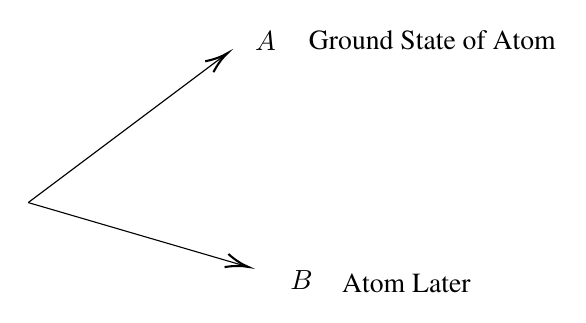
\begin{tikzpicture}[x=0.75pt,y=0.75pt,yscale=-1,xscale=1]
%uncomment if require: \path (0,300); %set diagram left start at 0, and has height of 300

%Straight Lines [id:da5358387187871396] 
\draw    (100,112) -- (194.4,41.2) ;
\draw [shift={(196,40)}, rotate = 143.13] [color={rgb, 255:red, 0; green, 0; blue, 0 }  ][line width=0.75]    (10.93,-3.29) .. controls (6.95,-1.4) and (3.31,-0.3) .. (0,0) .. controls (3.31,0.3) and (6.95,1.4) .. (10.93,3.29)   ;
%Straight Lines [id:da8208475664134449] 
\draw    (100,112) -- (204.08,142.44) ;
\draw [shift={(206,143)}, rotate = 196.3] [color={rgb, 255:red, 0; green, 0; blue, 0 }  ][line width=0.75]    (10.93,-3.29) .. controls (6.95,-1.4) and (3.31,-0.3) .. (0,0) .. controls (3.31,0.3) and (6.95,1.4) .. (10.93,3.29)   ;

% Text Node
\draw (225,143.4) node [anchor=north west][inner sep=0.75pt]    {$B$};
% Text Node
\draw (208,28.4) node [anchor=north west][inner sep=0.75pt]    {$A$};
% Text Node
\draw (234,28) node [anchor=north west][inner sep=0.75pt]   [align=left] {{\fontfamily{ptm}\selectfont Ground State of Atom}};
% Text Node
\draw (250,145) node [anchor=north west][inner sep=0.75pt]   [align=left] {{\fontfamily{ptm}\selectfont Atom Later}};


\end{tikzpicture}

\end{center}

\subsection{Legendre Polynomials}

(i) \mbox{} \\
HW1 $\rightarrow$ $\frac{1}{ \sqrt{1 - 2xt + t^2}} = \sum_{n=0}^{\infty} P_n(x)
t^n$ \mbox{} \\\\

\noindent (ii) \mbox{} \\

\[
  1, x, xnn^2, x^3, \dots \hspace{10px} \text{Gram Schmidt} \rightarrow P_0, P_1,
  P_2
\] \vspace{5px} 
\[
\langle \hspace{2px} P_n \hspace{2px} | \hspace{2px} P_n \hspace{2px} \rangle
= \int_{-1}^{1} P_n (x) P_m(x) dx = 0 \hspace{10px} \text{if } m \neq n
\] \vspace{5px} \mbox{} \\\\

\noindent (iii) \mbox{} \\
Solving 2nd Order ODE (Legendre's Eqn / Laplace's PDE)


\subsection{Rank of a Matrix}

\begin{tcolorbox}[colback = blue!5!white, colframe = blue!50!black, title
  = Example 1]
  
  \begin{align*}
    &x + y = 3 \\
    & 7x + 4y = 11 
  \end{align*}
\[
  \begin{pmatrix}
    1 & 1 & 3 \\
    7 & 7 & 11
  \end{pmatrix} \rightarrow 
  \begin{pmatrix}
    1 & 1 & 3 \\
    0 & 0 & -10
  \end{pmatrix} \rightarrow \text{ No Soln } 
\]
\end{tcolorbox}

\begin{tcolorbox}[colback = red!5!white, colframe = red!50!black, title
  = Example 2]
  
  \begin{align*}
    & x + y = 3 \\
    & 7x + 7y = 21
  \end{align*}

  \[
  \begin{pmatrix}
    1 & 1 & 3 \\
    7 & 7 & 21
  \end{pmatrix} \rightarrow 
  \begin{pmatrix}
    1 & 1 & 3 \\ 
    0 & 0 & 0
  \end{pmatrix} \rightarrow \text{infinite solutions}
  \] \vspace{5px} 
  \begin{align*}
    &x + y = 3 \\
    &0 + 0 = 0
  \end{align*} 
  
\end{tcolorbox}

\begin{tcolorbox}[colback = blue!5!white, colframe = blue!50!black, title
  = General]
  
  \[
  A \rightarrow 
  \begin{pmatrix}
    1 & 0 & 0 & \dots \\
    0 & 1 & 0 & \\
    0 & 0 & 1 & \\
    0 & 0 & 0 & \ddots \\ 
    \vdots &  & 
  \end{pmatrix}
  \] \vspace{5px} 
  
 Rank A $ = 4$ 

\end{tcolorbox}

Rank of a Matrix is the \# of non-zero rows \textbf{after} row reduction. 


\section{Determinants}

Objective: How to determine if system of vectors are linearly dependent or
not. 
\[
  \vec{A}, \vec{B}, \vec{C} \hspace{10px} \text{linearly dependent?}
\] \vspace{5px} 
\[
\alpha \vec{A} + \beta \vec{B} + \gamma \vec{C} = 0  
\] \vspace{5px} 
\[
\alpha
\begin{pmatrix}
  a_1 \\ a_2\\ a_3
\end{pmatrix} + 
\beta
\begin{pmatrix}
  b_1 \\ b_2 \\ 3 
\end{pmatrix} + 
\gamma 
\begin{pmatrix}
  c_1 \\ c_2 \\ c_3 
\end{pmatrix} = \vec{0}
\] \vspace{5px} 
\[
M = \begin{pmatrix} 
  a_1 & b_1 & c_1  \\
  a_2 & b_2 & c_2 \\
  a_3 & b_3 & c_3  
\end{pmatrix} 
\] \vspace{5px} 

Is $\det M = 0?$

\[
 2D \hspace{10px} \vec{A}, \vec{B} \text{ is linearly independent if } \det M \neq 0 
\] \vspace{5px} 

\paragraph{Calculating Determinant} \mbox{} \\

1. Einstein Levi Civita Tensor: 

\[
  (\vec{A} \times \vec{B} ) \cdot \vec{C} = \sum_i \sum_j \sum_k A_i B_j C_k
\] \vspace{5px} 
2. Row Operations \mbox{} \\

3. Calculate it normally: 

\[
\det \begin{pmatrix} 
a_1 & b_1 & c_1 \\
a_2 & b_2 & c_2 \\
c_1 & c_2 & c_3 
\end{pmatrix} 
\] \vspace{5px}

\paragraph{Properties of Determinants} \mbox{} \\

\begin{itemize}
  \item $\det(M^T) = \det M$
  \item $\det (AB) = (\det A)(\det B)$
\end{itemize}
\vspace{5px}
\textbf{Row Operations} \mbox{} \\
(1) \\
\[
\begin{vmatrix} 
a_1 & a_2 & a_3 \\ 
b_1 & b_2 & b_3 \\
c_1 & c_2 & c_3 
\end{vmatrix}  = 
- \begin{vmatrix} 
a_1 & a_2 & a_3 \\ 
c_1 & c_2 & c_3 \\
b_1 & b_2 & b_3 
\end{vmatrix} 
\] \vspace{5px} 

\[
  (\vec{C} \times \vec{B}) \cdot \vec{A} = - (\vec{A} \times \vec{B} ) \cdot
  \vec{C}
\] \vspace{5px} 
(2) \\
\[
\begin{vmatrix} 
a_1 & a_2 & a_3 \ 
\lambda b_1 & \lambda b_2 & \lambda b_3 \ 
c_1 & c_2 & c_3 
\end{vmatrix} = \lambda \begin{vmatrix} 
a_1 & a_2 & a_3 \\
b_1 & b_2 & b_3 \\
c_1 & c_2 & c_3 
\end{vmatrix} \mbox{} \\
\] \vspace{5px} 


\paragraph{Algorithm to compute Determinant} \mbox{} \\

\begin{itemize}
  \item perform row operations keep track of (-) signs and constants
    multiplied. 
\end{itemize}




\end{document}  

